\documentclass{standalone}
\usepackage{tikz}
\usetikzlibrary{patterns, angles}

\begin{document}
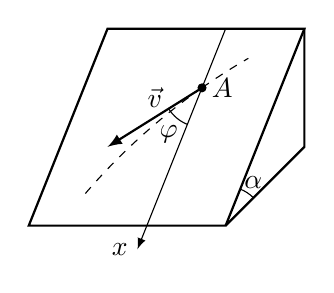
\begin{tikzpicture}
	\coordinate (A) at (0, 0);
    \coordinate (B) at (2.5, 0);
    \coordinate (C) at (3.5, 1);
    \coordinate (D) at (3.5, 2.5);
    \coordinate (E) at (1, 2.5);
    \coordinate (F) at (2.2, 1.75);
    \coordinate (G) at (1.38,-0.3);
    \coordinate (H) at (1,1);
    
	\draw [thick] (A) -- (B) -- (D) -- (E) -- cycle;
	\draw [thick] (B) -- (C) -- (D);

	\draw [arrows={-latex}] (2.5,2.5) -- (G) node [left] {$x$};
	\draw [fill] (2.2, 1.75) circle (0.05) node [right] {$A$};
	\draw [thick, arrows={-latex}] (F)--(H) node [midway, above] {$\vec{v}$}; 
	\pic [draw, -, angle eccentricity=1.5] {angle = H--F--G};
	\node [left=12pt, below=10pt] at (F) {$\varphi$};	
	
	\draw [dashed] (F) arc (125:140:8);	
	\draw [dashed] (F) arc (125:120:8);

	\pic [draw, -, angle eccentricity=1.5] {angle = C--B--D};
	\node [right=10pt, above=10pt] at (B) {$\alpha$};
\end{tikzpicture}
\end{document}